\chapter{掃引線アルゴリズム - Sweep line algorithms}

\index{掃引線 - sweep line}

幾何学的な問題のいくつかは、\key{掃引線 - sweep line}を用いたアルゴリズムで解くことができます。
これは問題を、平面上の点に対応するイベントの集合として表現するアイデアです。
イベントは、その$x$または$y$に従って昇順に処理します。

例えば、従業員数$n$人の会社があり、
各従業員のある日の出社・退社時刻が わかっているとします。
我々の仕事は、同時にオフィスにいた 従業員の最大人数を計算することです。

この問題は、各従業員に出社時間と退社時間に対応する2つのイベントを割り当てるようにして解決できます。
イベントを分類した後、そのイベントを調べて、オフィスにいる人数を把握します。

例を示します。

\begin{center}
\begin{tabular}{ccc}
名前 & 出社 & 退社 \\
\hline
John & 10 & 15 \\
Maria & 6 & 12 \\
Peter & 14 & 16 \\
Lisa & 5 & 13 \\
\end{tabular}
\end{center}
これは次のようなイベントです。
\begin{center}
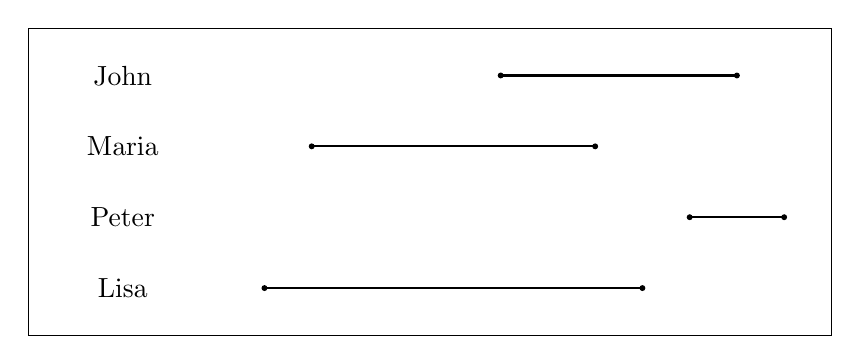
\begin{tikzpicture}[scale=0.6]
\draw (0,0) rectangle (17,-6.5);
\path[draw,thick,-] (10,-1) -- (15,-1);
\path[draw,thick,-] (6,-2.5) -- (12,-2.5);
\path[draw,thick,-] (14,-4) -- (16,-4);
\path[draw,thick,-] (5,-5.5) -- (13,-5.5);

\draw[fill] (10,-1) circle [radius=0.05];
\draw[fill] (15,-1) circle [radius=0.05];
\draw[fill] (6,-2.5) circle [radius=0.05];
\draw[fill] (12,-2.5) circle [radius=0.05];
\draw[fill] (14,-4) circle [radius=0.05];
\draw[fill] (16,-4) circle [radius=0.05];
\draw[fill] (5,-5.5) circle [radius=0.05];
\draw[fill] (13,-5.5) circle [radius=0.05];

\node at (2,-1) {John};
\node at (2,-2.5) {Maria};
\node at (2,-4) {Peter};
\node at (2,-5.5) {Lisa};
\end{tikzpicture}
\end{center}
このとき、左から右へイベントを辿り、カウンタを管理します。
出社イベントの時、カウンタをインクリメントします。
退社イベントの時はカウンタをデクリメントします。
こうすると答えはその間の最大値になります。

この例では次のように処理が行われます。
\begin{center}
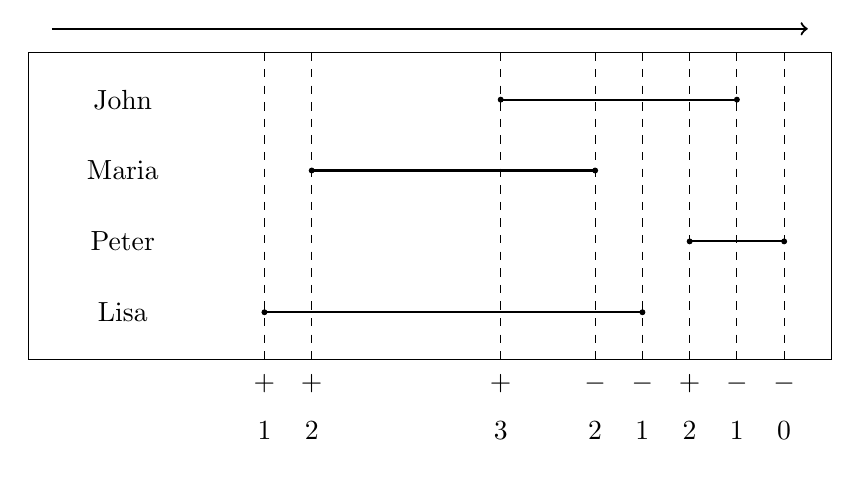
\begin{tikzpicture}[scale=0.6]
\path[draw,thick,->] (0.5,0.5) -- (16.5,0.5);
\draw (0,0) rectangle (17,-6.5);
\path[draw,thick,-] (10,-1) -- (15,-1);
\path[draw,thick,-] (6,-2.5) -- (12,-2.5);
\path[draw,thick,-] (14,-4) -- (16,-4);
\path[draw,thick,-] (5,-5.5) -- (13,-5.5);

\draw[fill] (10,-1) circle [radius=0.05];
\draw[fill] (15,-1) circle [radius=0.05];
\draw[fill] (6,-2.5) circle [radius=0.05];
\draw[fill] (12,-2.5) circle [radius=0.05];
\draw[fill] (14,-4) circle [radius=0.05];
\draw[fill] (16,-4) circle [radius=0.05];
\draw[fill] (5,-5.5) circle [radius=0.05];
\draw[fill] (13,-5.5) circle [radius=0.05];

\node at (2,-1) {John};
\node at (2,-2.5) {Maria};
\node at (2,-4) {Peter};
\node at (2,-5.5) {Lisa};

\path[draw,dashed] (10,0)--(10,-6.5);
\path[draw,dashed] (15,0)--(15,-6.5);
\path[draw,dashed] (6,0)--(6,-6.5);
\path[draw,dashed] (12,0)--(12,-6.5);
\path[draw,dashed] (14,0)--(14,-6.5);
\path[draw,dashed] (16,0)--(16,-6.5);
\path[draw,dashed] (5,0)--(5,-6.5);
\path[draw,dashed] (13,0)--(13,-6.5);

\node at (10,-7) {$+$};
\node at (15,-7) {$-$};
\node at (6,-7) {$+$};
\node at (12,-7) {$-$};
\node at (14,-7) {$+$};
\node at (16,-7) {$-$};
\node at (5,-7) {$+$};
\node at (13,-7) {$-$};

\node at (10,-8) {$3$};
\node at (15,-8) {$1$};
\node at (6,-8) {$2$};
\node at (12,-8) {$2$};
\node at (14,-8) {$2$};
\node at (16,-8) {$0$};
\node at (5,-8) {$1$};
\node at (13,-8) {$1$};
\end{tikzpicture}
\end{center}

各記号はカウンターの値が増加するか減少するかを示し、
カウンターの値は記号の下に示すようになります。
カウンターの最大値は、ジョンが到着してからマリアが帰るまでの間の3です。

イベントのソートに$O(n \log n)$の時間がかかり、残りのアルゴリズムに
$O(n)$の時間がかかるため、このアルゴリズムの実行時間は$O(n \log n)$である。

\section{交差点 - Intersection points}

\index{交差点 - intersection point}


各々が水平または垂直な$n$本の線分の集合があるとき、交点の総数を数える問題を考えましょう。

\begin{center}
\begin{tikzpicture}[scale=0.5]
\path[draw,thick,-] (0,2) -- (5,2);
\path[draw,thick,-] (1,4) -- (6,4);
\path[draw,thick,-] (6,3) -- (10,3);
\path[draw,thick,-] (2,1) -- (2,6);
\path[draw,thick,-] (8,2) -- (8,5);
\end{tikzpicture}
\end{center}
この場合の交差点は3つです。
\begin{center}
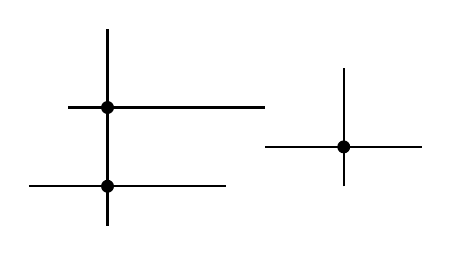
\begin{tikzpicture}[scale=0.5]
\path[draw,thick,-] (0,2) -- (5,2);
\path[draw,thick,-] (1,4) -- (6,4);
\path[draw,thick,-] (6,3) -- (10,3);
\path[draw,thick,-] (2,1) -- (2,6);
\path[draw,thick,-] (8,2) -- (8,5);

\draw[fill] (2,2) circle [radius=0.15];
\draw[fill] (2,4) circle [radius=0.15];
\draw[fill] (8,3) circle [radius=0.15];

\end{tikzpicture}
\end{center}

この問題を$O(n^2)$時間で解くのは簡単です。
全ての線分の組を調べて、それらが交差しているかどうかをチェックします。
しかし、掃引線アルゴリズムと区間クエリデータ構造を用いれば、
$O(n \log n)$の時間で解けます。
線分の端点を左から右へ処理し、次の3種類の事象に注目するというものです。

\begin{enumerate}[noitemsep]
\item[(1)] 水平線の開始
\item[(2)] 水平線の終了
\item[(3)] 垂直線
\end{enumerate}

先ほどの例では次のようなイベントの対応になります。
\begin{center}
\begin{tikzpicture}[scale=0.6]
\path[draw,dashed] (0,2) -- (5,2);
\path[draw,dashed] (1,4) -- (6,4);
\path[draw,dashed] (6,3) -- (10,3);
\path[draw,dashed] (2,1) -- (2,6);
\path[draw,dashed] (8,2) -- (8,5);

\node at (0,2) {$1$};
\node at (5,2) {$2$};
\node at (1,4) {$1$};
\node at (6,4) {$2$};
\node at (6,3) {$1$};
\node at (10,3) {$2$};

\node at (2,3.5) {$3$};
\node at (8,3.5) {$3$};
\end{tikzpicture}
\end{center}

イベントを左から右へみていき、
アクティブな水平線が存在する$y$座標のセットを保持するデータ構造を持ちます。
イベント1 では、セグメントの $y$ 座標をセットに追加し、
イベント2 では、その $y$ 座標をセットから削除します。

イベント3 を処理する時に交点を計算します。
点$y_1$と$y_2$ の間に垂直セグメントがある場合、
$y$座標が$y_1$ と$y_2$ の間にあるアクティブな水平セグメントの数を数え、
この数を交点の総数に加えればよいです。

水平線の $y$ 座標を格納するために、
BITまたは セグメントツリーを使用し、
場合によっては座標圧縮を行います。
このような構造を使用する場合、各イベントの処理に $O(\log n)$ の時間がかかるため、
アルゴリズムの総実行時間は $O(n \log n)$ となります。

\section{近接ペア問題 - Closest pair problem}

\index{近接ペア - closest pair}

$n$個の点の集合が与えられ、ユークリッド距離が最小となる2点を見つける問題を考えます。
例えば、点が
\begin{center}
\begin{tikzpicture}[scale=0.7]
\draw (0,0)--(12,0)--(12,4)--(0,4)--(0,0);

\draw (1,2) circle [radius=0.1];
\draw (3,1) circle [radius=0.1];
\draw (4,3) circle [radius=0.1];
\draw (5.5,1.5) circle [radius=0.1];
\draw (6,2.5) circle [radius=0.1];
\draw (7,1) circle [radius=0.1];
\draw (9,1.5) circle [radius=0.1];
\draw (10,2) circle [radius=0.1];
\draw (1.5,3.5) circle [radius=0.1];
\draw (1.5,1) circle [radius=0.1];
\draw (2.5,3) circle [radius=0.1];
\draw (4.5,1.5) circle [radius=0.1];
\draw (5.25,0.5) circle [radius=0.1];
\draw (6.5,2) circle [radius=0.1];
\end{tikzpicture}
\end{center}
\begin{samepage}
のとき、以下の2点を見つけます。
\begin{center}
\begin{tikzpicture}[scale=0.7]
\draw (0,0)--(12,0)--(12,4)--(0,4)--(0,0);

\draw (1,2) circle [radius=0.1];
\draw (3,1) circle [radius=0.1];
\draw (4,3) circle [radius=0.1];
\draw (5.5,1.5) circle [radius=0.1];
\draw[fill] (6,2.5) circle [radius=0.1];
\draw (7,1) circle [radius=0.1];
\draw (9,1.5) circle [radius=0.1];
\draw (10,2) circle [radius=0.1];
\draw (1.5,3.5) circle [radius=0.1];
\draw (1.5,1) circle [radius=0.1];
\draw (2.5,3) circle [radius=0.1];
\draw (4.5,1.5) circle [radius=0.1];
\draw (5.25,0.5) circle [radius=0.1];
\draw[fill] (6.5,2) circle [radius=0.1];
\end{tikzpicture}
\end{center}
\end{samepage}

これも掃引線アルゴリズムを用いると
$O(n \log n)$ の時間で解ける問題の一例です
\footnote{Besides this approach,
there is also an
$O(n \log n)$ time divide-and-conquer algorithm \cite{sha75}
that divides the points into two sets and recursively
solves the problem for both sets.}。
左から右へと点を巡り、これまでに見た2点間の最小距離である値dを保持します。
このとき各点で、左側に最も近い点を探します。
その距離が$d$より小さい場合、それが新しい最小距離となり、$d$の値を更新します。

現在の点が$(x, y)$として、左側に$d$以下の距離に点がある場合、
その点のx座標は$[x-d,x]$の間でなければなく、
y座標は$[y-d,y+d]$の間でなければなりません。
そのため、これらの範囲に位置する点のみを考慮すれば十分であり、
このアルゴリズムは効率的に動作します。

例えば、以下の図において破線で示した領域は、
現在の値からd以内の距離に存在しうる点を表すことになります。

\begin{center}
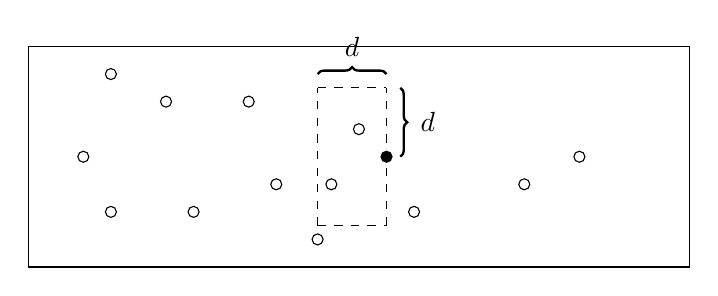
\begin{tikzpicture}[scale=0.7]
\draw (0,0)--(12,0)--(12,4)--(0,4)--(0,0);

\draw (1,2) circle [radius=0.1];
\draw (3,1) circle [radius=0.1];
\draw (4,3) circle [radius=0.1];
\draw (5.5,1.5) circle [radius=0.1];
\draw (6,2.5) circle [radius=0.1];
\draw (7,1) circle [radius=0.1];
\draw (9,1.5) circle [radius=0.1];
\draw (10,2) circle [radius=0.1];
\draw (1.5,3.5) circle [radius=0.1];
\draw (1.5,1) circle [radius=0.1];
\draw (2.5,3) circle [radius=0.1];
\draw (4.5,1.5) circle [radius=0.1];
\draw (5.25,0.5) circle [radius=0.1];
\draw[fill] (6.5,2) circle [radius=0.1];

\draw[dashed] (6.5,0.75)--(6.5,3.25);
\draw[dashed] (5.25,0.75)--(5.25,3.25);
\draw[dashed] (5.25,0.75)--(6.5,0.75);
\draw[dashed] (5.25,3.25)--(6.5,3.25);

\draw [decoration={brace}, decorate, line width=0.3mm] (5.25,3.5) -- (6.5,3.5);
\node at (5.875,4) {$d$};
\draw [decoration={brace}, decorate, line width=0.3mm] (6.75,3.25) -- (6.75,2);
\node at (7.25,2.625) {$d$};
\end{tikzpicture}
\end{center}


このアルゴリズムが効率的に動くのは、
各領域には常に$O(1)$個の点しか含まれないという事実に基づいています。
$x$座標が$[x-d,x]$の間にある点の集合を、
$y$座標に従って昇順に保持することにより、
$O(\log n)$時間でそれらの点を走査することができるのです。

このアルゴリズムの時間計算量は$O(n \log n)$です。
$n$の各点について左に最も近い点を$O(\log n)$時間で求められます。

\section{凸包問題 - Convex hull problem}

\key{凸包 - convex hull}とは、
与えられた集合のすべての点を含む最小の凸の多角形のことです。
凸とは、多角形の任意の2つの頂点を結ぶ線分が完全にある多角形の内部にあることを意味します。

\begin{samepage}
例えば以下の点を考えます。
\begin{center}
\begin{tikzpicture}[scale=0.7]
\draw (0,0) circle [radius=0.1];
\draw (4,-1) circle [radius=0.1];
\draw (7,1) circle [radius=0.1];
\draw (6,3) circle [radius=0.1];
\draw (2,4) circle [radius=0.1];
\draw (0,2) circle [radius=0.1];

\draw (1,1) circle [radius=0.1];
\draw (2,2) circle [radius=0.1];
\draw (3,2) circle [radius=0.1];
\draw (4,0) circle [radius=0.1];
\draw (4,3) circle [radius=0.1];
\draw (5,2) circle [radius=0.1];
\draw (6,1) circle [radius=0.1];
\end{tikzpicture}
\end{center}
\end{samepage}
この時の凸包は
\begin{center}
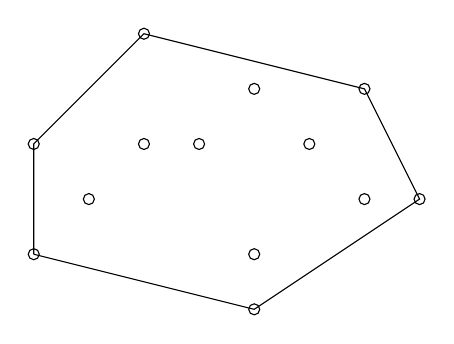
\begin{tikzpicture}[scale=0.7]
\draw (0,0)--(4,-1)--(7,1)--(6,3)--(2,4)--(0,2)--(0,0);

\draw (0,0) circle [radius=0.1];
\draw (4,-1) circle [radius=0.1];
\draw (7,1) circle [radius=0.1];
\draw (6,3) circle [radius=0.1];
\draw (2,4) circle [radius=0.1];
\draw (0,2) circle [radius=0.1];

\draw (1,1) circle [radius=0.1];
\draw (2,2) circle [radius=0.1];
\draw (3,2) circle [radius=0.1];
\draw (4,0) circle [radius=0.1];
\draw (4,3) circle [radius=0.1];
\draw (5,2) circle [radius=0.1];
\draw (6,1) circle [radius=0.1];
\end{tikzpicture}
\end{center}

\index{アンドリューのアルゴリズム - Andrew's algorithm}

\key{アンドリューのアルゴリズム - Andrew's algorithm} \cite{and79}
は、点群に対する凸包を$O(n \log n)$時間構成するアルゴリズムです。
このアルゴリズムでは,まず左端と右端の点を求め,凸包を上包と下包の2つに分けます。
このとき、まず上部の構築に集中します。

まず、点を主に$x$座標で、次に$y$座標の順で並べ替えます。
その後、各ポイントを凸包に追加していきます。
点を追加した後は、常に、凸包の最後の線分が左に曲がらないようにします。
左に曲がっているならば、最後から2つ目の点を凸包から取り除いていきます。
以下の図は、Andrewのアルゴリズムがどのように動作するかを示しています。

\begin{tabular}{ccccccc}
\\
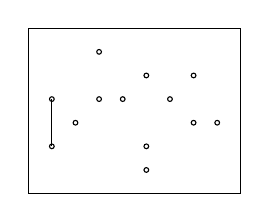
\begin{tikzpicture}[scale=0.3]
\draw (-1,-2)--(8,-2)--(8,5)--(-1,5)--(-1,-2);
\draw (0,0) circle [radius=0.1];
\draw (4,-1) circle [radius=0.1];
\draw (7,1) circle [radius=0.1];
\draw (6,3) circle [radius=0.1];
\draw (2,4) circle [radius=0.1];
\draw (0,2) circle [radius=0.1];

\draw (1,1) circle [radius=0.1];
\draw (2,2) circle [radius=0.1];
\draw (3,2) circle [radius=0.1];
\draw (4,0) circle [radius=0.1];
\draw (4,3) circle [radius=0.1];
\draw (5,2) circle [radius=0.1];
\draw (6,1) circle [radius=0.1];

\draw (0,0)--(0,2);
\end{tikzpicture}
& \hspace{0.1cm} &
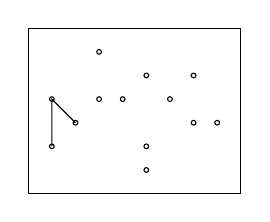
\begin{tikzpicture}[scale=0.3]
\draw (-1,-2)--(8,-2)--(8,5)--(-1,5)--(-1,-2);
\draw (0,0) circle [radius=0.1];
\draw (4,-1) circle [radius=0.1];
\draw (7,1) circle [radius=0.1];
\draw (6,3) circle [radius=0.1];
\draw (2,4) circle [radius=0.1];
\draw (0,2) circle [radius=0.1];

\draw (1,1) circle [radius=0.1];
\draw (2,2) circle [radius=0.1];
\draw (3,2) circle [radius=0.1];
\draw (4,0) circle [radius=0.1];
\draw (4,3) circle [radius=0.1];
\draw (5,2) circle [radius=0.1];
\draw (6,1) circle [radius=0.1];

\draw (0,0)--(0,2)--(1,1);
\end{tikzpicture}
& \hspace{0.1cm} &
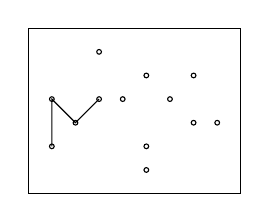
\begin{tikzpicture}[scale=0.3]
\draw (-1,-2)--(8,-2)--(8,5)--(-1,5)--(-1,-2);
\draw (0,0) circle [radius=0.1];
\draw (4,-1) circle [radius=0.1];
\draw (7,1) circle [radius=0.1];
\draw (6,3) circle [radius=0.1];
\draw (2,4) circle [radius=0.1];
\draw (0,2) circle [radius=0.1];

\draw (1,1) circle [radius=0.1];
\draw (2,2) circle [radius=0.1];
\draw (3,2) circle [radius=0.1];
\draw (4,0) circle [radius=0.1];
\draw (4,3) circle [radius=0.1];
\draw (5,2) circle [radius=0.1];
\draw (6,1) circle [radius=0.1];

\draw (0,0)--(0,2)--(1,1)--(2,2);
\end{tikzpicture}
& \hspace{0.1cm} &
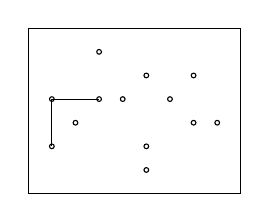
\begin{tikzpicture}[scale=0.3]
\draw (-1,-2)--(8,-2)--(8,5)--(-1,5)--(-1,-2);
\draw (0,0) circle [radius=0.1];
\draw (4,-1) circle [radius=0.1];
\draw (7,1) circle [radius=0.1];
\draw (6,3) circle [radius=0.1];
\draw (2,4) circle [radius=0.1];
\draw (0,2) circle [radius=0.1];

\draw (1,1) circle [radius=0.1];
\draw (2,2) circle [radius=0.1];
\draw (3,2) circle [radius=0.1];
\draw (4,0) circle [radius=0.1];
\draw (4,3) circle [radius=0.1];
\draw (5,2) circle [radius=0.1];
\draw (6,1) circle [radius=0.1];

\draw (0,0)--(0,2)--(2,2);
\end{tikzpicture}
\\
1 & & 2 & & 3 & & 4 \\
\end{tabular}
\\
\begin{tabular}{ccccccc}
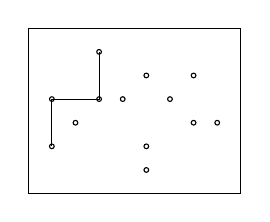
\begin{tikzpicture}[scale=0.3]
\draw (-1,-2)--(8,-2)--(8,5)--(-1,5)--(-1,-2);
\draw (0,0) circle [radius=0.1];
\draw (4,-1) circle [radius=0.1];
\draw (7,1) circle [radius=0.1];
\draw (6,3) circle [radius=0.1];
\draw (2,4) circle [radius=0.1];
\draw (0,2) circle [radius=0.1];

\draw (1,1) circle [radius=0.1];
\draw (2,2) circle [radius=0.1];
\draw (3,2) circle [radius=0.1];
\draw (4,0) circle [radius=0.1];
\draw (4,3) circle [radius=0.1];
\draw (5,2) circle [radius=0.1];
\draw (6,1) circle [radius=0.1];

\draw (0,0)--(0,2)--(2,2)--(2,4);
\end{tikzpicture}
& \hspace{0.1cm} &
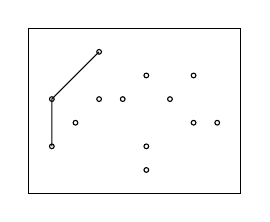
\begin{tikzpicture}[scale=0.3]
\draw (-1,-2)--(8,-2)--(8,5)--(-1,5)--(-1,-2);
\draw (0,0) circle [radius=0.1];
\draw (4,-1) circle [radius=0.1];
\draw (7,1) circle [radius=0.1];
\draw (6,3) circle [radius=0.1];
\draw (2,4) circle [radius=0.1];
\draw (0,2) circle [radius=0.1];

\draw (1,1) circle [radius=0.1];
\draw (2,2) circle [radius=0.1];
\draw (3,2) circle [radius=0.1];
\draw (4,0) circle [radius=0.1];
\draw (4,3) circle [radius=0.1];
\draw (5,2) circle [radius=0.1];
\draw (6,1) circle [radius=0.1];

\draw (0,0)--(0,2)--(2,4);
\end{tikzpicture}
& \hspace{0.1cm} &
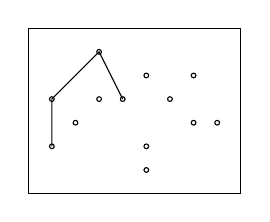
\begin{tikzpicture}[scale=0.3]
\draw (-1,-2)--(8,-2)--(8,5)--(-1,5)--(-1,-2);
\draw (0,0) circle [radius=0.1];
\draw (4,-1) circle [radius=0.1];
\draw (7,1) circle [radius=0.1];
\draw (6,3) circle [radius=0.1];
\draw (2,4) circle [radius=0.1];
\draw (0,2) circle [radius=0.1];

\draw (1,1) circle [radius=0.1];
\draw (2,2) circle [radius=0.1];
\draw (3,2) circle [radius=0.1];
\draw (4,0) circle [radius=0.1];
\draw (4,3) circle [radius=0.1];
\draw (5,2) circle [radius=0.1];
\draw (6,1) circle [radius=0.1];

\draw (0,0)--(0,2)--(2,4)--(3,2);
\end{tikzpicture}
& \hspace{0.1cm} &
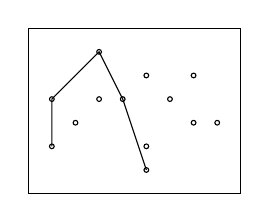
\begin{tikzpicture}[scale=0.3]
\draw (-1,-2)--(8,-2)--(8,5)--(-1,5)--(-1,-2);
\draw (0,0) circle [radius=0.1];
\draw (4,-1) circle [radius=0.1];
\draw (7,1) circle [radius=0.1];
\draw (6,3) circle [radius=0.1];
\draw (2,4) circle [radius=0.1];
\draw (0,2) circle [radius=0.1];

\draw (1,1) circle [radius=0.1];
\draw (2,2) circle [radius=0.1];
\draw (3,2) circle [radius=0.1];
\draw (4,0) circle [radius=0.1];
\draw (4,3) circle [radius=0.1];
\draw (5,2) circle [radius=0.1];
\draw (6,1) circle [radius=0.1];

\draw (0,0)--(0,2)--(2,4)--(3,2)--(4,-1);
\end{tikzpicture}
\\
5 & & 6 & & 7 & & 8 \\
\end{tabular}
\\
\begin{tabular}{ccccccc}
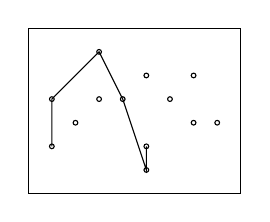
\begin{tikzpicture}[scale=0.3]
\draw (-1,-2)--(8,-2)--(8,5)--(-1,5)--(-1,-2);
\draw (0,0) circle [radius=0.1];
\draw (4,-1) circle [radius=0.1];
\draw (7,1) circle [radius=0.1];
\draw (6,3) circle [radius=0.1];
\draw (2,4) circle [radius=0.1];
\draw (0,2) circle [radius=0.1];

\draw (1,1) circle [radius=0.1];
\draw (2,2) circle [radius=0.1];
\draw (3,2) circle [radius=0.1];
\draw (4,0) circle [radius=0.1];
\draw (4,3) circle [radius=0.1];
\draw (5,2) circle [radius=0.1];
\draw (6,1) circle [radius=0.1];

\draw (0,0)--(0,2)--(2,4)--(3,2)--(4,-1)--(4,0);
\end{tikzpicture}
& \hspace{0.1cm} &
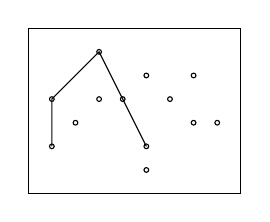
\begin{tikzpicture}[scale=0.3]
\draw (-1,-2)--(8,-2)--(8,5)--(-1,5)--(-1,-2);
\draw (0,0) circle [radius=0.1];
\draw (4,-1) circle [radius=0.1];
\draw (7,1) circle [radius=0.1];
\draw (6,3) circle [radius=0.1];
\draw (2,4) circle [radius=0.1];
\draw (0,2) circle [radius=0.1];

\draw (1,1) circle [radius=0.1];
\draw (2,2) circle [radius=0.1];
\draw (3,2) circle [radius=0.1];
\draw (4,0) circle [radius=0.1];
\draw (4,3) circle [radius=0.1];
\draw (5,2) circle [radius=0.1];
\draw (6,1) circle [radius=0.1];

\draw (0,0)--(0,2)--(2,4)--(3,2)--(4,0);
\end{tikzpicture}
& \hspace{0.1cm} &
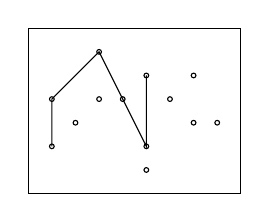
\begin{tikzpicture}[scale=0.3]
\draw (-1,-2)--(8,-2)--(8,5)--(-1,5)--(-1,-2);
\draw (0,0) circle [radius=0.1];
\draw (4,-1) circle [radius=0.1];
\draw (7,1) circle [radius=0.1];
\draw (6,3) circle [radius=0.1];
\draw (2,4) circle [radius=0.1];
\draw (0,2) circle [radius=0.1];

\draw (1,1) circle [radius=0.1];
\draw (2,2) circle [radius=0.1];
\draw (3,2) circle [radius=0.1];
\draw (4,0) circle [radius=0.1];
\draw (4,3) circle [radius=0.1];
\draw (5,2) circle [radius=0.1];
\draw (6,1) circle [radius=0.1];

\draw (0,0)--(0,2)--(2,4)--(3,2)--(4,0)--(4,3);
\end{tikzpicture}
& \hspace{0.1cm} &
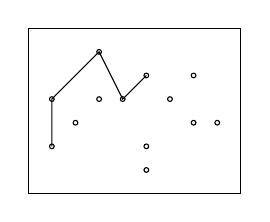
\begin{tikzpicture}[scale=0.3]
\draw (-1,-2)--(8,-2)--(8,5)--(-1,5)--(-1,-2);
\draw (0,0) circle [radius=0.1];
\draw (4,-1) circle [radius=0.1];
\draw (7,1) circle [radius=0.1];
\draw (6,3) circle [radius=0.1];
\draw (2,4) circle [radius=0.1];
\draw (0,2) circle [radius=0.1];

\draw (1,1) circle [radius=0.1];
\draw (2,2) circle [radius=0.1];
\draw (3,2) circle [radius=0.1];
\draw (4,0) circle [radius=0.1];
\draw (4,3) circle [radius=0.1];
\draw (5,2) circle [radius=0.1];
\draw (6,1) circle [radius=0.1];

\draw (0,0)--(0,2)--(2,4)--(3,2)--(4,3);
\end{tikzpicture}
\\
9 & & 10 & & 11 & & 12 \\
\end{tabular}
\\
\begin{tabular}{ccccccc}
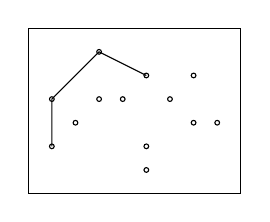
\begin{tikzpicture}[scale=0.3]
\draw (-1,-2)--(8,-2)--(8,5)--(-1,5)--(-1,-2);
\draw (0,0) circle [radius=0.1];
\draw (4,-1) circle [radius=0.1];
\draw (7,1) circle [radius=0.1];
\draw (6,3) circle [radius=0.1];
\draw (2,4) circle [radius=0.1];
\draw (0,2) circle [radius=0.1];

\draw (1,1) circle [radius=0.1];
\draw (2,2) circle [radius=0.1];
\draw (3,2) circle [radius=0.1];
\draw (4,0) circle [radius=0.1];
\draw (4,3) circle [radius=0.1];
\draw (5,2) circle [radius=0.1];
\draw (6,1) circle [radius=0.1];

\draw (0,0)--(0,2)--(2,4)--(4,3);
\end{tikzpicture}
& \hspace{0.1cm} &
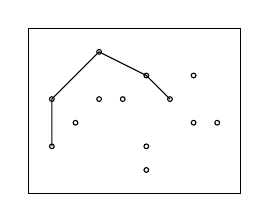
\begin{tikzpicture}[scale=0.3]
\draw (-1,-2)--(8,-2)--(8,5)--(-1,5)--(-1,-2);
\draw (0,0) circle [radius=0.1];
\draw (4,-1) circle [radius=0.1];
\draw (7,1) circle [radius=0.1];
\draw (6,3) circle [radius=0.1];
\draw (2,4) circle [radius=0.1];
\draw (0,2) circle [radius=0.1];

\draw (1,1) circle [radius=0.1];
\draw (2,2) circle [radius=0.1];
\draw (3,2) circle [radius=0.1];
\draw (4,0) circle [radius=0.1];
\draw (4,3) circle [radius=0.1];
\draw (5,2) circle [radius=0.1];
\draw (6,1) circle [radius=0.1];

\draw (0,0)--(0,2)--(2,4)--(4,3)--(5,2);
\end{tikzpicture}
& \hspace{0.1cm} &
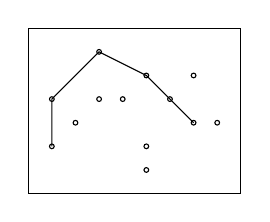
\begin{tikzpicture}[scale=0.3]
\draw (-1,-2)--(8,-2)--(8,5)--(-1,5)--(-1,-2);
\draw (0,0) circle [radius=0.1];
\draw (4,-1) circle [radius=0.1];
\draw (7,1) circle [radius=0.1];
\draw (6,3) circle [radius=0.1];
\draw (2,4) circle [radius=0.1];
\draw (0,2) circle [radius=0.1];

\draw (1,1) circle [radius=0.1];
\draw (2,2) circle [radius=0.1];
\draw (3,2) circle [radius=0.1];
\draw (4,0) circle [radius=0.1];
\draw (4,3) circle [radius=0.1];
\draw (5,2) circle [radius=0.1];
\draw (6,1) circle [radius=0.1];

\draw (0,0)--(0,2)--(2,4)--(4,3)--(5,2)--(6,1);
\end{tikzpicture}
& \hspace{0.1cm} &
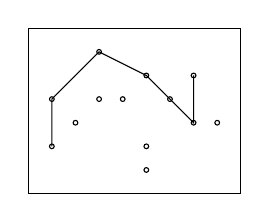
\begin{tikzpicture}[scale=0.3]
\draw (-1,-2)--(8,-2)--(8,5)--(-1,5)--(-1,-2);
\draw (0,0) circle [radius=0.1];
\draw (4,-1) circle [radius=0.1];
\draw (7,1) circle [radius=0.1];
\draw (6,3) circle [radius=0.1];
\draw (2,4) circle [radius=0.1];
\draw (0,2) circle [radius=0.1];

\draw (1,1) circle [radius=0.1];
\draw (2,2) circle [radius=0.1];
\draw (3,2) circle [radius=0.1];
\draw (4,0) circle [radius=0.1];
\draw (4,3) circle [radius=0.1];
\draw (5,2) circle [radius=0.1];
\draw (6,1) circle [radius=0.1];

\draw (0,0)--(0,2)--(2,4)--(4,3)--(5,2)--(6,1)--(6,3);
\end{tikzpicture}
\\
13 & & 14 & & 15 & & 16 \\
\end{tabular}
\\
\begin{tabular}{ccccccc}
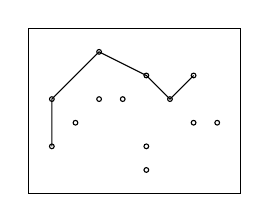
\begin{tikzpicture}[scale=0.3]
\draw (-1,-2)--(8,-2)--(8,5)--(-1,5)--(-1,-2);
\draw (0,0) circle [radius=0.1];
\draw (4,-1) circle [radius=0.1];
\draw (7,1) circle [radius=0.1];
\draw (6,3) circle [radius=0.1];
\draw (2,4) circle [radius=0.1];
\draw (0,2) circle [radius=0.1];

\draw (1,1) circle [radius=0.1];
\draw (2,2) circle [radius=0.1];
\draw (3,2) circle [radius=0.1];
\draw (4,0) circle [radius=0.1];
\draw (4,3) circle [radius=0.1];
\draw (5,2) circle [radius=0.1];
\draw (6,1) circle [radius=0.1];

\draw (0,0)--(0,2)--(2,4)--(4,3)--(5,2)--(6,3);
\end{tikzpicture}
& \hspace{0.1cm} &
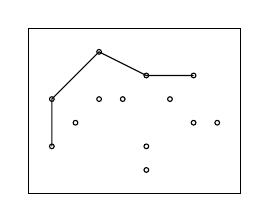
\begin{tikzpicture}[scale=0.3]
\draw (-1,-2)--(8,-2)--(8,5)--(-1,5)--(-1,-2);
\draw (0,0) circle [radius=0.1];
\draw (4,-1) circle [radius=0.1];
\draw (7,1) circle [radius=0.1];
\draw (6,3) circle [radius=0.1];
\draw (2,4) circle [radius=0.1];
\draw (0,2) circle [radius=0.1];

\draw (1,1) circle [radius=0.1];
\draw (2,2) circle [radius=0.1];
\draw (3,2) circle [radius=0.1];
\draw (4,0) circle [radius=0.1];
\draw (4,3) circle [radius=0.1];
\draw (5,2) circle [radius=0.1];
\draw (6,1) circle [radius=0.1];

\draw (0,0)--(0,2)--(2,4)--(4,3)--(6,3);
\end{tikzpicture}
& \hspace{0.1cm} &
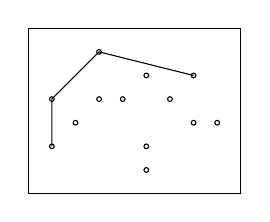
\begin{tikzpicture}[scale=0.3]
\draw (-1,-2)--(8,-2)--(8,5)--(-1,5)--(-1,-2);
\draw (0,0) circle [radius=0.1];
\draw (4,-1) circle [radius=0.1];
\draw (7,1) circle [radius=0.1];
\draw (6,3) circle [radius=0.1];
\draw (2,4) circle [radius=0.1];
\draw (0,2) circle [radius=0.1];

\draw (1,1) circle [radius=0.1];
\draw (2,2) circle [radius=0.1];
\draw (3,2) circle [radius=0.1];
\draw (4,0) circle [radius=0.1];
\draw (4,3) circle [radius=0.1];
\draw (5,2) circle [radius=0.1];
\draw (6,1) circle [radius=0.1];

\draw (0,0)--(0,2)--(2,4)--(6,3);
\end{tikzpicture}
& \hspace{0.1cm} &
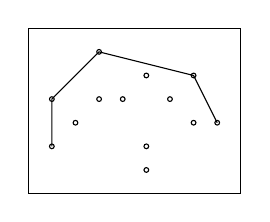
\begin{tikzpicture}[scale=0.3]
\draw (-1,-2)--(8,-2)--(8,5)--(-1,5)--(-1,-2);
\draw (0,0) circle [radius=0.1];
\draw (4,-1) circle [radius=0.1];
\draw (7,1) circle [radius=0.1];
\draw (6,3) circle [radius=0.1];
\draw (2,4) circle [radius=0.1];
\draw (0,2) circle [radius=0.1];

\draw (1,1) circle [radius=0.1];
\draw (2,2) circle [radius=0.1];
\draw (3,2) circle [radius=0.1];
\draw (4,0) circle [radius=0.1];
\draw (4,3) circle [radius=0.1];
\draw (5,2) circle [radius=0.1];
\draw (6,1) circle [radius=0.1];

\draw (0,0)--(0,2)--(2,4)--(6,3)--(7,1);
\end{tikzpicture}
\\
17 & & 18 & & 19 & & 20
\end{tabular}
